\chapter{Relation Between Two Continuous Variables}

If we have two related variables, the \emph{correlation} measures the association between the two variables. In contrast, a \emph{linear regression} is used for the prediction of the value of one variable from another. If we want to compare more than two groups of variables, we have to use a technique known as \emph{Analysis of Variance (ANOVA)}.

\section{Correlation}

\subsection{Correlation Coefficient} \index{general}{correlation coefficient}

If the two variables are normally distributed, the standard measure of determining the \emph{correlation coefficient}, often ascribed to \emph{Pearson} \index{general}{correlation!Pearson}, is

\begin{equation}\label{eq:pearson}
  r = \frac{\sum\limits_{i=1}^n (X_i - \bar{X})(Y_i - \bar{Y})}{\sqrt{\sum\limits_{i=1}^n (X_i - \bar{X})^2} \sqrt{\sum\limits_{i=1}^n (Y_i - \bar{Y})^2}}
\end{equation}

With

\begin{equation}
  s_{xy} = \frac{\sum\limits_{i=1}^n (X_i - \bar{X})(Y_i - \bar{Y})}{n-1}
\end{equation}

and $s_x, s_y$ the sample standard deviations of the $x$ and $y$ values, respectively, the Equation \ref{eq:pearson} can also be written as

\begin{equation}
  r = \frac{s_{xy}}{s_x \cdot s_y}.
\end{equation}

Pearson's correlation coefficient, sometimes also referred to as \emph{population correlation coefficient} or \emph{sample correlation}, can take any value from -1 to +1. Examples are given in Figure \ref{fig:correlation}. Note that the formula for the correlation coefficient is symmetrical between $x$ and $y$.

\subsection{Coefficient of determination}

The \emph{coefficient of determination} \index{general}{coefficient of determination} or $R^2$ is the square of the correlation. It is easier to interpret than the correlation coefficient r: Values of $R^2$ close to 1 are good, values close to 0 are poor. To explain the interpretation of $R^2$, let us look at the math more formally:

\begin{figure}
  \centering
  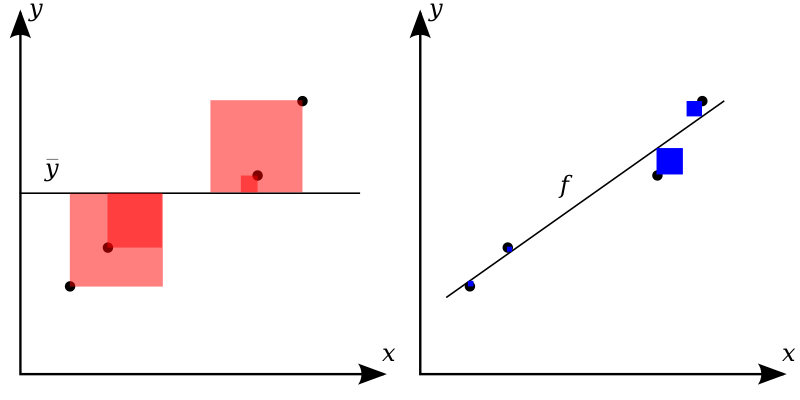
\includegraphics[width=0.75\textwidth]{../Images/Coefficient_of_Determination.png}\\
  \caption{The better the linear regression (on the right) fits the data in comparison to the simple average (on the left graph), the closer the value of $R^2$ is to one. The areas of the blue squares represent the squared residuals with respect to the linear regression. The areas of the red squares represent the squared residuals with respect to the average value (from Wikipedia)}\label{fig:CoefDetermination}
\end{figure}

A data set has values $y_i$, each of which has an associated modelled value $f_i$ (also sometimes referred to as $\hat{y}_i$). Here, the values $y_i$ are called the \emph{observed values}* and the modelled values $f_i$ are sometimes called the \emph{predicted values}.

In the following $\bar{y}$ is the mean of the observed data:

\begin{equation}
  \bar{y}=\frac{1}{n}\sum_{i=1}^n y_i
\end{equation}

where n is the number of observations.

The "variability" of the data set is measured through different sums of squares:

    $SS_\text{tot}=\sum_i (y_i-\bar{y})^2$, the total sum of squares (proportional to the sample variance);

    $SS_\text{reg}=\sum_i (f_i -\bar{y})^2$, the regression sum of squares, also called the explained sum of squares.

    $SS_\text{res}=\sum_i (y_i - f_i)^2\,$, the sum of squares of residuals, also called the residual sum of squares.

The notations $SS_{R}$ and $SS_{E}$ should be avoided, since in some texts their meaning is reversed to "Residual sum of squares" and "Explained sum of squares", respectively.

The most general definition of the coefficient of determination is

\begin{equation}
  R^2 \equiv 1 - {SS_{\rm res}\over SS_{\rm tot}}.\,
\end{equation}

\subsubsection{Relation to unexplained variance}

In a general form, $R^2$ can be seen to be related to the unexplained variance, since the second term compares the unexplained variance (variance of the model's errors) with the total variance (of the data). See fraction of variance unexplained.

\subsubsection{Adjusted $R^2$}\index{general}{coefficient of determination!adjusted}

For multiple regression, the \emph{adjusted $R^2$} value (written as $\bar{R}^2$) is often used instead of $R^2$:

\begin{equation}\label{eq:adjustedR2}
      \bar{R}^2 = 1 - (1 - R^2)\frac{n - 1}{n - p - 1}
\end{equation}

where $n$ is the sample size and $p$ is the number of independent variables.

\begin{figure}
  \centering
  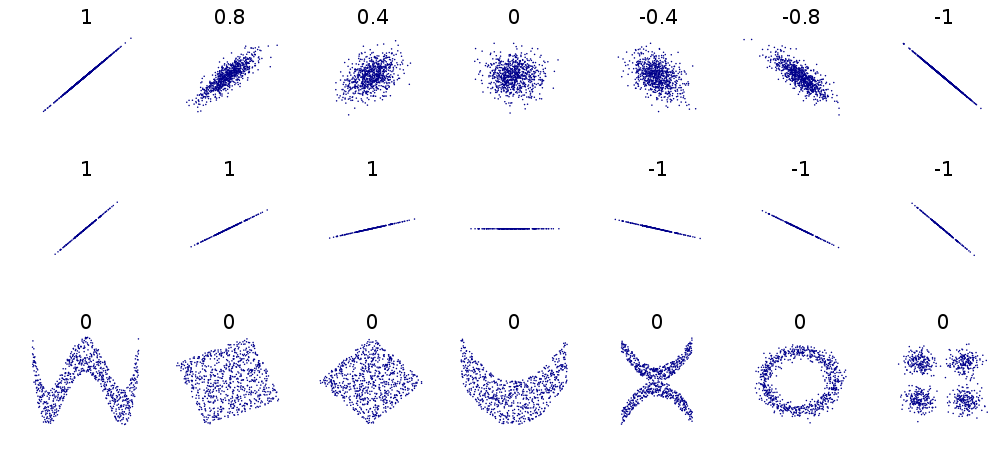
\includegraphics[width=0.75\textwidth]{../Images/Correlation_examples2.png}\\
  \caption{Several sets of (x, y) points, with the correlation coefficient of x and y for each set. Note that the correlation reflects the non-linearity and direction of a linear relationship (top row), but not the slope of that relationship (middle), nor many aspects of nonlinear relationships (bottom). N.B.: the figure in the center has a slope of 0 but in that case the correlation coefficient is undefined because the variance of Y is zero. (From: Wikipedia)}\label{fig:correlation}
\end{figure}

\subsubsection{Examples}

How large $R^2$ or $\bar{R}^2$ must be to be considered good depends on the discipline. They are usually expected to be larger in the physical sciences than it is in biology or the social sciences. In finance or marketing, it also depends on what is being modeled.

Caution: the sample correlation and $R^2$ are misleading if there is a nonlinear relationship between the independent and dependent variables!

\subsection{Rank Correlation}

If the data distribution is not normal, a different approach is necessary. In that case one can rank the set of subjects for each variable and compare the orderings. There are two commonly used methods of calculating the rank correlation. \index{general}{correlation!Spearman}
\index{general}{correlation!Kendall's $\tau$}

\begin{itemize}
  \item   \emph{Spearman's $\rho$}, which is exactly the same as the Pearson correlation coefficient $r$ calculated on the ranks of the observations.
  \item   \emph{Kendall's $\tau$} is also a rank correlation coefficient, measuring the association between two measured quantities. It is harder to calculate than Spearman's rho, but it has been argued that confidence intervals for Spearman’s rho are less reliable and less interpretable than confidence intervals for Kendall’s tau-parameters.
\end{itemize}

%\begin{itemize}
%  \item   "Regression to the mean"
%  \item   Partial correlation (comment)
%\end{itemize}

%(Lecture 11)

\section{Regression} \index{general}{regression}

We can use the method of \emph{regression} when we want to predict the value of one variable from the other.

\begin{figure}
  \centering
  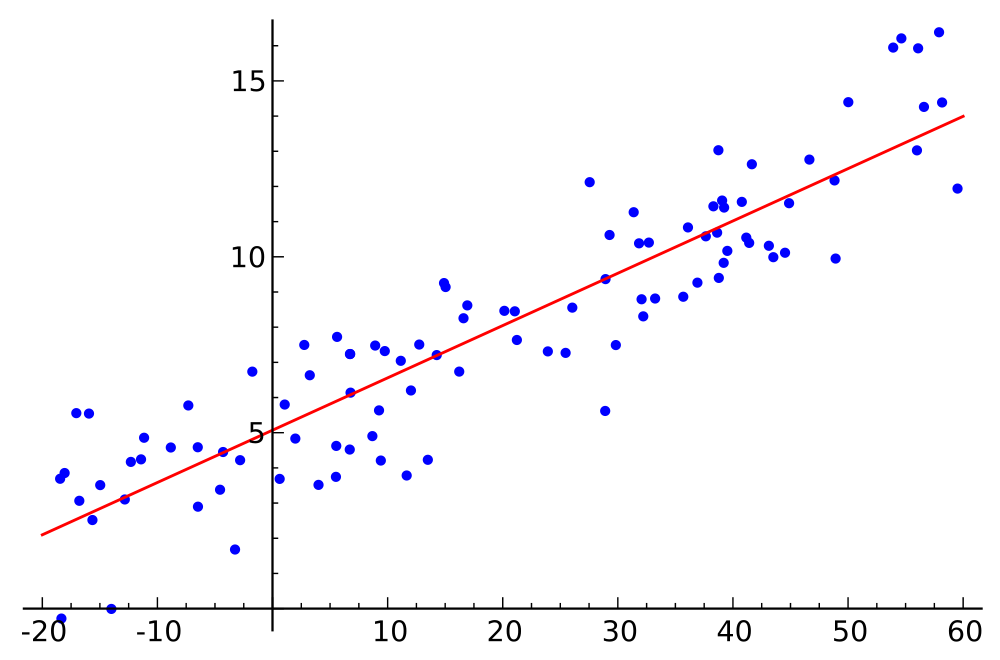
\includegraphics[width=0.75\textwidth]{../Images/Linear_regression.png}\\
  \caption{Linear regression. (From Wikipedia)}\label{fig:regression}
\end{figure}

When we search for the best-fit line to a given $(x_i,y_i)$ dataset, we are looking for the parameters $(k,d)$ which minimize the sum of the squared \emph{residuals} $\epsilon_i$ in

\begin{equation}\label{eq:simpleRegression}
  y_i = k * x_i + d + \epsilon_i
\end{equation}

where $k$ is the \emph{slope} or \emph{inclination} of the line, and $d$ the \emph{intercept}. This is in fact just the one-dimensional example of the more general technique, which is described in the next section.
Note that in contrast to the correlation, this relationship between $x$ and $y$ is no more symmetrical: it is assumed that the $x-$values are known exactly, and that all the variability lies in the residuals.

\begin{figure}
  \centering
  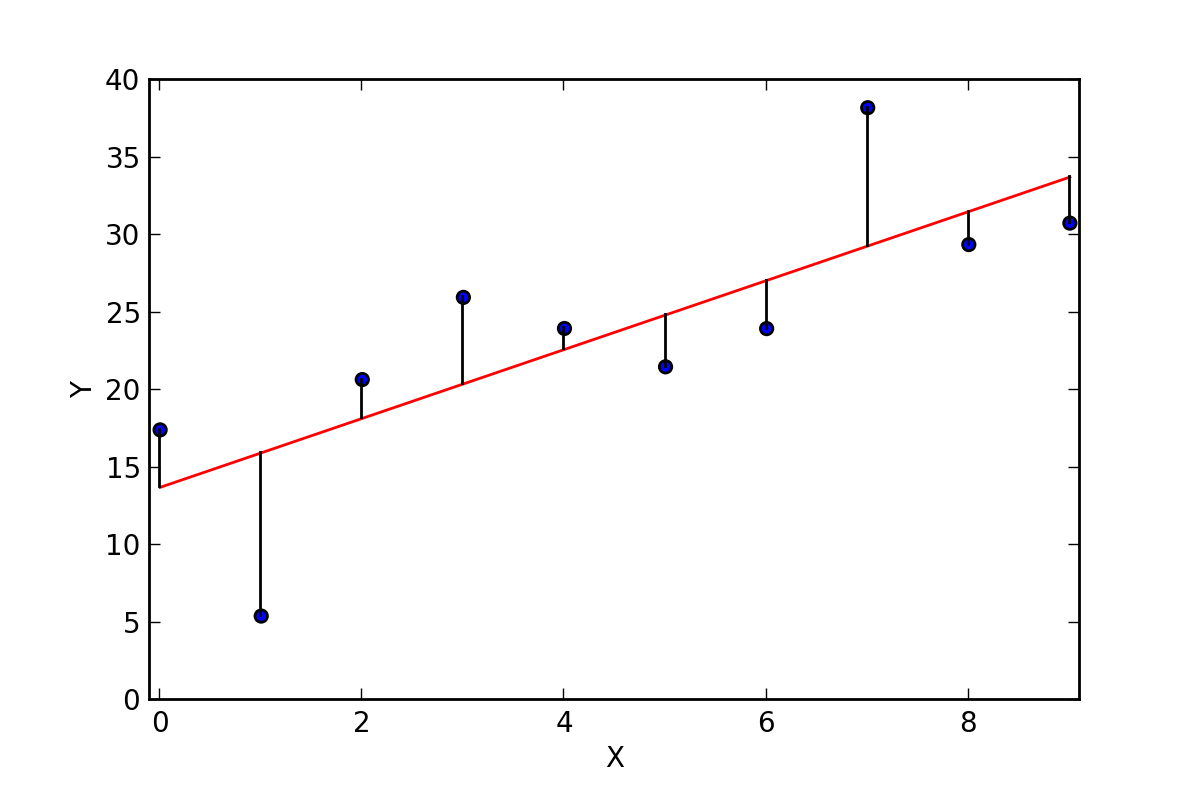
\includegraphics[width=0.75\textwidth]{../Images/residuals_linreg.png}\\
  \caption{Best-fit linear regression line (red) and residuals (black). }\label{fig:residuals}
\end{figure}


\subsection{Introduction}

\footnote{This section has been taken from Wikipedia} Given a data set $\{y_i,\, x_{i1}, \ldots, x_{ip}\}_{i=1}^n$ of $n$ statistical units, a linear regression model assumes that the relationship between the dependent variable $y_i$ and the $p$-vector of regressors $x_i$ is linear. This relationship is modelled through a \emph{disturbance term} or \emph{error variable} $\epsilon_i$, an unobserved random variable that adds noise to the linear relationship between the dependent variable and regressors. Thus the model takes the form

\begin{equation}\label{eq:regression}
   y_i = \beta_1   x_{i1} + \cdots + \beta_p x_{ip} + \varepsilon_i
   = \mathbf{x}^{\rm T}_i\boldsymbol\beta + \varepsilon_i,
   \qquad i = 1, \ldots, n,
\end{equation}

where $^T$ denotes the transpose, so that $x_i^T\beta$ is the inner product between vectors $x_i$ $\beta$.

Often these $n$ equations are stacked together and written in vector form as

\begin{equation}
  \mathbf{y} = \mathbf{X}\boldsymbol\beta + \boldsymbol\varepsilon, \,
\end{equation}

where

\begin{equation}
   \mathbf{y} = \begin{pmatrix} y_1 \\ y_2 \\ \vdots \\ y_n \end{pmatrix}, \quad
   \mathbf{X} = \begin{pmatrix} \mathbf{x}^{\rm T}_1 \\ \mathbf{x}^{\rm T}_2 \\ \vdots \\ \mathbf{x}^{\rm T}_n \end{pmatrix}
   = \begin{pmatrix} x_{11} & \cdots & x_{1p} \\
   x_{21} & \cdots & x_{2p} \\
   \vdots & \ddots & \vdots \\
   x_{n1} & \cdots & x_{np}
   \end{pmatrix}, \quad
   \boldsymbol\beta = \begin{pmatrix} \beta_1 \\ \vdots \\ \beta_p \end{pmatrix}, \quad
   \boldsymbol\varepsilon = \begin{pmatrix} \varepsilon_1 \\ \varepsilon_2 \\ \vdots \\ \varepsilon_n \end{pmatrix}.
\end{equation}

Some remarks on terminology and general use:
\begin{itemize} \index{general}{covariate} \index{general}{regressand} \index{general}{endogenous variable} \index{general}{regressor} \index{general}{exogenous variable}
  \item $y_i$  is called the \emph{regressand}, \emph{endogenous variable}, \emph{response variable}, \emph{measured variable}, or \emph{dependent variable}.  The decision as to which variable in a data set is modeled as the dependent variable and which are modeled as the independent variables may be based on a presumption that the value of one of the variables is caused by, or directly influenced by the other variables. Alternatively, there may be an operational reason to model one of the variables in terms of the others, in which case there need be no presumption of causality.
  \item $\mathbf{x}_i$ are called \emph{regressors}, \emph{exogenous variables}, \emph{explanatory variables}, \emph{covariates}, \emph{input variables}, \emph{predictor variables}, or \emph{independent variables}, but not to be confused with \emph{independent random variables}. The matrix $\mathbf{X}$ is sometimes called the \emph{design matrix}.
      \begin{itemize}
        \item Usually a constant is included as one of the regressors. For example we can take $x_{i1}=1$ for $i=1,...,n$. The corresponding element of $\beta$ is called the \emph{intercept}. Many statistical inference procedures for linear models require an intercept to be present, so it is often included even if theoretical considerations suggest that its value should be zero.
        \item Sometimes one of the regressors can be a non-linear function of another regressor or of the data, as in polynomial regression and segmented regression. The model remains linear as long as it is linear in the parameter vector $\beta$.
        \item The regressors $x_{ij}$ may be viewed either as random variables, which we simply observe, or they can be considered as predetermined fixed values which we can choose. Both interpretations may be appropriate in different cases, and they generally lead to the same estimation procedures; however different approaches to asymptotic analysis are used in these two situations.
         \end{itemize}
  \item $\boldsymbol\beta\,$ is a $p$-dimensional \emph{parameter vector}. Its elements are also called \emph{effects}, or \emph{regression coefficients}. Statistical estimation and inference in linear regression focuses on $\beta$.
  \item $\varepsilon_i\,$ is called the \emph{residuals}, \emph{error term}, \emph{disturbance term}, or \emph{noise}. This variable captures all other factors which influence the dependent variable $y_i$ other than the regressors $x_i$. The relationship between the error term and the regressors, for example whether they are correlated, is a crucial step in formulating a linear regression model, as it will determine the method to use for estimation.
  \item If $i=1$ and $p=1$ in Eq.\ref{eq:regression}, we have a \emph{simple linear regression}, corresponding to Eq.\ref{eq:simpleRegression}. If $i>1$ we talk about \emph{multilinear regression} \index{general}{regression!multilinear} or \emph{multiple linear regression} \index{general}{regression!multiple linear|see{regression!multilinear}}.

\end{itemize}
\emph{Example}. Consider a situation where a small ball is being tossed up in the air and then we measure its heights of ascent $h_i$ at various moments in time $t_i$. Physics tells us that, ignoring the drag, the relationship can be modelled as
:

\begin{equation}
 h_i = \beta_1 t_i + \beta_2 t_i^2 + \varepsilon_i,
\end{equation}

where $\beta_1$ determines the initial velocity of the ball, $\beta_2$ is proportional to the standard gravity, and $\epsilon_i$ is due to measurement errors. Linear regression can be used to estimate the values of $\beta_1$ and $\beta_2$ from the measured data. This model is non-linear in the time variable, but it is linear in the parameters $\beta_1$ and $\beta_2$; if we take regressors $\mathbf{x}_i = (x_{i1},x_{i2}) = (t_i,t_i^2)$, the model takes on the standard form
:
 $h_i = \mathbf{x}^{\rm T}_i\boldsymbol\beta + \varepsilon_i.$

\subsection{Assumptions}

To use the technique of linear regression, the following assumptions should be fulfilled:

\begin{enumerate}
  \item The \emph{independent variables} (i.e. $x$) are exactly known.
  \item Validity. Most importantly, the data you are analyzing should map to the research question you are trying to answer. This sounds obvious but is often overlooked or ignored because it can be inconvenient. For example, a linear regression does not properly describe a quadratic curve.
  \item Additivity and linearity. The most important mathematical assumption of the regression model is that its deterministic component is a linear function of the separate predictors.
  \item Independence of errors.
  \item Equal variance of errors.
  \item Normality of errors.
\end{enumerate}

\begin{figure}
  \centering
  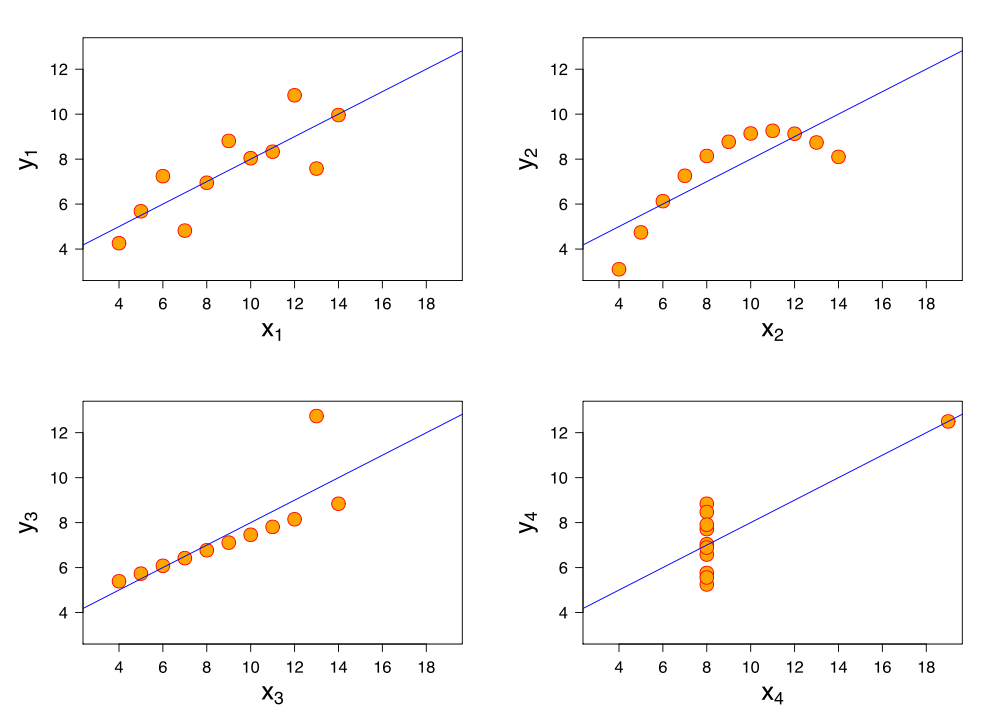
\includegraphics[width=0.75\textwidth]{../Images/Anscombes_quartet.png}\\
  \caption{The sets in the \emph{Anscombe's quartet} have the same linear regression line but are themselves very different.}
\end{figure}

\PyImg "multivariate.py" (p \pageref{py:multivariate}): Analysis of multivariate data (regression, correlation).
\index{python}{multivariate}

\begin{figure}
  \centering
  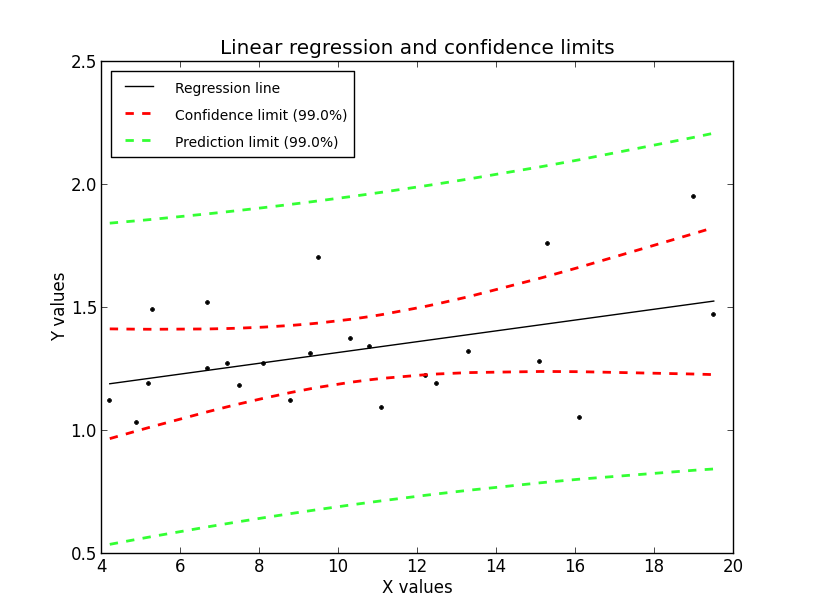
\includegraphics[width=0.75\textwidth]{../Images/regression_wLegend.png}\\
  \caption{Regression, with confidence intervals for the mean, as well as for the predicted data. The red dotted line shows the confidence interval for the mean; and the green dotted line the confidence interval for predicted data. (This can be compared to the standard error and the standard deviation for a population.)} \label{fig:regline}
\end{figure}

Since to my knowledge there exists no program in the Python standard library (or numpy, scipy) to calculate the confidence intervals for a regression line, I include my corresponding program \emph{lineFit.py} \ref{py:fitLine}. The output of this program is shown in Figure \ref{fig:regline}. This program also shows how Python programs intended for distribution should be documented.

\PyImg "fitLine.py" (p \pageref{py:fitLine}): Linear regression fit.
\index{python}{fitLine}

\section{Exercises}

\begin{enumerate}
  \item \textbf{Correlation}

    Read in the data for the average yearly temperature at the Sonnblick, from     \emph{https://github.com/thomas-haslwanter/statsintro/blob/master/Data/data\_others/AvgTemp.xls}
    Calculate the Pearson and Spearman correlation, and Kendall's tau, for the temperature vs. year.

  \item \textbf{Regression}

    For the same data, calculate the yearly increase in temperature, assuming a linear increase with time.
    Is this increase significant?

  \item \textbf{Normality Check}

    For the data from the regression model, check if the model is ok by testing if the residuals are normally distributed (e.g. by using the Kolmogorov-Smirnov test)

\end{enumerate}


